\documentclass[11pt,a4paper]{article}
\usepackage[margin=2.4cm]{geometry}
\usepackage{fontspec}
\usepackage{booktabs}
\usepackage{graphicx}
\usepackage{float}
\usepackage[table]{xcolor}
\usepackage[colorlinks=true,linkcolor=black,urlcolor=blue,citecolor=black]{hyperref}

% parskip / caption / enumitem are not in a minimal TeX install, so the few
% settings taken from them are written out here instead. This keeps the report
% compilable with nothing but a base TeX Live.
\setlength{\parindent}{0pt}
\setlength{\parskip}{0.55em}
\setlength{\abovecaptionskip}{6pt}
\setlength{\belowcaptionskip}{2pt}

\newfontfamily\gujaratifont{Gujarati Sangam MN}[Scale=1.05]
\newfontfamily\nepalifont{Devanagari Sangam MN}[Scale=1.05]
\newfontfamily\fallbackfont{Helvetica}
\newcommand{\gujaratitext}[1]{{\gujaratifont #1}}
\newcommand{\nepalitext}[1]{{\nepalifont #1}}
\newcommand{\fallbacktext}[1]{{\fallbackfont #1}}

\makeatletter
\renewcommand{\@makecaption}[2]{%
  \vskip\abovecaptionskip
  \begingroup\small #1: #2\par\endgroup
  \vskip\belowcaptionskip}
\makeatother
\setlength{\emergencystretch}{3em}

\title{\vspace{-1.5cm}\textbf{Phase 2 --- Model Implementation, Pretraining and
Evaluation}\\[0.3em]
\large Monolingual Transformer Language Models for Gujarati and Nepali}
\author{Language Models and Agents --- Individual Project}
\date{Branch \texttt{phase-2}}


\begin{document}

\maketitle

\vspace{-0.8cm}

\section{What was built}


Two decoder-only Transformer language models, written from scratch in PyTorch
and pretrained independently: \textbf{Model H} on Gujarati (higher-resource) and
\textbf{Model L} on Nepali (lower-resource). They share no data, no tokenizer,
no vocabulary and no weights. They do share an architecture and a training
recipe on purpose, so that the only variables between them are the corpus and
the tokenizer.

No \texttt{nn.Transformer*}, no HuggingFace model class and no
\texttt{F.scaled\_dot\_product\_attention}: attention, the causal mask and the
positional scheme are written out in \texttt{<language>/model/transformer.py}.


\begin{table}[H]
\centering
\small
\begin{tabular}{lrrrrr}
\toprule
\textbf{Model} & \textbf{Parameters} & \textbf{Vocabulary} & \textbf{Training tokens} & \textbf{Test PPL} & \textbf{Test BPB} \\
\midrule
Gujarati (Model H) & 25,625,856 & 16,000 & 518,586,368 & 51.62 & \textbf{0.5764} \\
Nepali (Model L) & 25,625,856 & 16,000 & 490,274,816 & 38.93 & \textbf{0.4247} \\
\bottomrule
\end{tabular}
\caption{Headline result. Bits-per-byte is the number that compares across two tokenizers; perplexity is per token and does not.}
\label{tab:summary}
\end{table}



\textbf{Checkpoints.} All ten --- five runs, each with \texttt{best.pt} (lowest
validation loss) and \texttt{latest.pt} (end of the run) --- are published at
\begin{center}
\url{https://huggingface.co/hardik300/LMA\_mini\_project}
\end{center}


\section{The model}


The forward pass is: token embedding $\rightarrow$ embedding dropout
$\rightarrow$ $N$ blocks of [LayerNorm $\rightarrow$ causal self-attention
$\rightarrow$ residual; LayerNorm $\rightarrow$ SwiGLU feed-forward
$\rightarrow$ residual] $\rightarrow$ final LayerNorm $\rightarrow$ tied output
projection $\rightarrow$ logits, trained with cross-entropy against the next
token.

Multi-head attention splits $(B,T,d)$ into $(B,h,T,d_k)$ with $d_k=d/h=64$,
computes $\mathrm{softmax}\!\left(QK^{\top}/\sqrt{d_k} + M\right)V$ per head,
then concatenates and applies $W_O$. The $1/\sqrt{d_k}$ scaling matters because
the dot product of two $d_k$-dimensional vectors grows like $d_k$; without it the
softmax saturates and its gradient vanishes. $M$ is an additive mask with
$-\infty$ above the diagonal, so position $t$ can only attend to positions
$\le t$.


\begin{table}[H]
\centering
\small
\begin{tabular}{lrr}
\toprule
\textbf{} & \textbf{Gujarati (Model H)} & \textbf{Nepali (Model L)} \\
\midrule
Model dimension $d$ & 384 & 384 \\
Layers $N$ & 11 & 11 \\
Attention heads $h$ & 6 & 6 \\
Feed-forward width & 1,024 & 1,024 \\
Context length $T$ & 512 & 512 \\
Vocabulary $V$ & 16,000 & 16,000 \\
\textbf{Parameters (total)} & \textbf{25,625,856} & \textbf{25,625,856} \\
\textbf{Parameters (non-embedding)} & \textbf{19,481,856} & \textbf{19,481,856} \\
\bottomrule
\end{tabular}
\caption{Architecture. Head dimension is $d/h = 64$. The two models are the same network with separate weights; only the vocabularies were built independently, and both sweeps chose 16{,}000.}
\label{tab:arch}
\end{table}



\textbf{Depth against width.} Phase 1 fixed $d=384$ by pricing the embedding
against the 25M budget. At that width one block costs 1{,}771{,}008 parameters,
so what is left after the 6.14M embedding buys 11 of them. The alternatives at
the same budget are wider and shallower ($448\times8$) or narrower and deeper
($320\times14$). Depth/width ratios of 20--40 behave similarly at this scale;
$384\times11$ sits in that band and trains faster than the narrow option, which
needs more sequential kernel launches for the same arithmetic --- which matters
on a single T4 with a fixed session limit.


\begin{table}[H]
\centering
\small
\begin{tabular}{p{0.16\linewidth}p{0.20\linewidth}p{0.52\linewidth}}
\toprule
\textbf{Choice} & \textbf{Setting} & \textbf{Reason} \\
\midrule
Positional scheme & RoPE & Costs no parameters (a learned table needs $512\times384=196{,}608$) and encodes relative distance, so length is not fixed by a table. \\
Normalisation & Pre-norm LayerNorm & Leaves an unbroken identity path through the stack, so 11 layers train without a long warmup. \\
Feed-forward & SwiGLU, $d_{ff}=1024$ & Same cost as GELU at 1536; the gate can suppress a channel multiplicatively. \\
Output head & Tied to the embedding & Saves 6.14M parameters, a quarter of the budget. \\
Biases & None & LayerNorm already re-centres every sublayer input. \\
Dropout & 0.0 for pretraining & One pass over ${\sim}500$M tokens: no document repeats, so there is nothing to memorise. Implemented and used in Phase 3. \\
Run length & One epoch & One pass is ${\sim}500$M tokens, which is both the brief's target and about 20 tokens per parameter. \\
\bottomrule
\end{tabular}
\caption{Design decisions and why they were made.}
\label{tab:decisions}
\end{table}


\subsection{Maximum sequence length}


RoPE stores no positional table, so the model does not fail on a longer
sequence: the cosine cache is recomputed for any length, and the self-test feeds
the trained architecture a 640-token input successfully. What is still bounded is
\emph{quality} --- the model never saw relative distances beyond 512, so it
degrades past that rather than raising an error. A learned table would have no
row for position 600 at all.


\subsection{Verifying the causal mask}


A model that can see the next token trains normally and reports an implausibly
low perplexity, so the mask is tested four ways in
\texttt{eval/causal\_check.py} instead of being assumed. The fourth is the
strongest: it differentiates a logit at position $t$ with respect to the input
embeddings and checks that no gradient reaches any position after $t$, which
tests the computational graph rather than just the values.


\begin{table}[H]
\centering
\small
\begin{tabular}{lrr}
\toprule
\textbf{Check} & \textbf{Gujarati} & \textbf{Nepali} \\
\midrule
Future edit moves earlier logits & 0.0e+00 \textsc{pass} & 0.0e+00 \textsc{pass} \\
Prefix vs.\ full-sequence logits differ & 0.0e+00 \textsc{pass} & 0.0e+00 \textsc{pass} \\
Largest weight above the diagonal & 0.0e+00 \textsc{pass} & 0.0e+00 \textsc{pass} \\
Gradient reaching a future position & 0.0e+00 \textsc{pass} & 0.0e+00 \textsc{pass} \\
\bottomrule
\end{tabular}
\caption{Causal masking, verified empirically rather than assumed. A model that could see the next token would train normally and report an implausibly low perplexity.}
\label{tab:causal}
\end{table}


\section{Pretraining}


Each model was trained for one epoch over its own tokenized training split on a
single Kaggle T4, in fp16 with a gradient scaler. Checkpoints contain model
weights, optimizer state, scheduler state, scaler state, step, tokens seen, both
configs and the RNG states, so a run resumes exactly where it stopped; the batch
order is a function of (seed, step) alone, so a resumed run continues on the data
it would have seen anyway.


\begin{table}[H]
\centering
\small
\begin{tabular}{lrr}
\toprule
\textbf{} & \textbf{Gujarati (Model H)} & \textbf{Nepali (Model L)} \\
\midrule
Optimizer steps & 15,826 & 14,962 \\
Training tokens seen & 518,586,368 & 490,274,816 \\
Wall-clock hours (Kaggle T4) & 4.57 & 4.51 \\
Throughput (tokens/s, median) & 31,738 & 30,497 \\
Final training loss & 3.9837 & 3.6508 \\
Best validation loss & 3.9450 & 3.6667 \\
\bottomrule
\end{tabular}
\caption{Pretraining. Both runs used AdamW ($\beta=(0.9,0.95)$, weight decay 0.1 on matrices only), 500 warmup steps then cosine decay from $6\times10^{-4}$ to $6\times10^{-5}$, gradient clipping at 1.0, batch $32\times2\times512=32{,}768$ tokens, seed 1337.}
\label{tab:pretrain}
\end{table}


\begin{figure}[H]
\centering
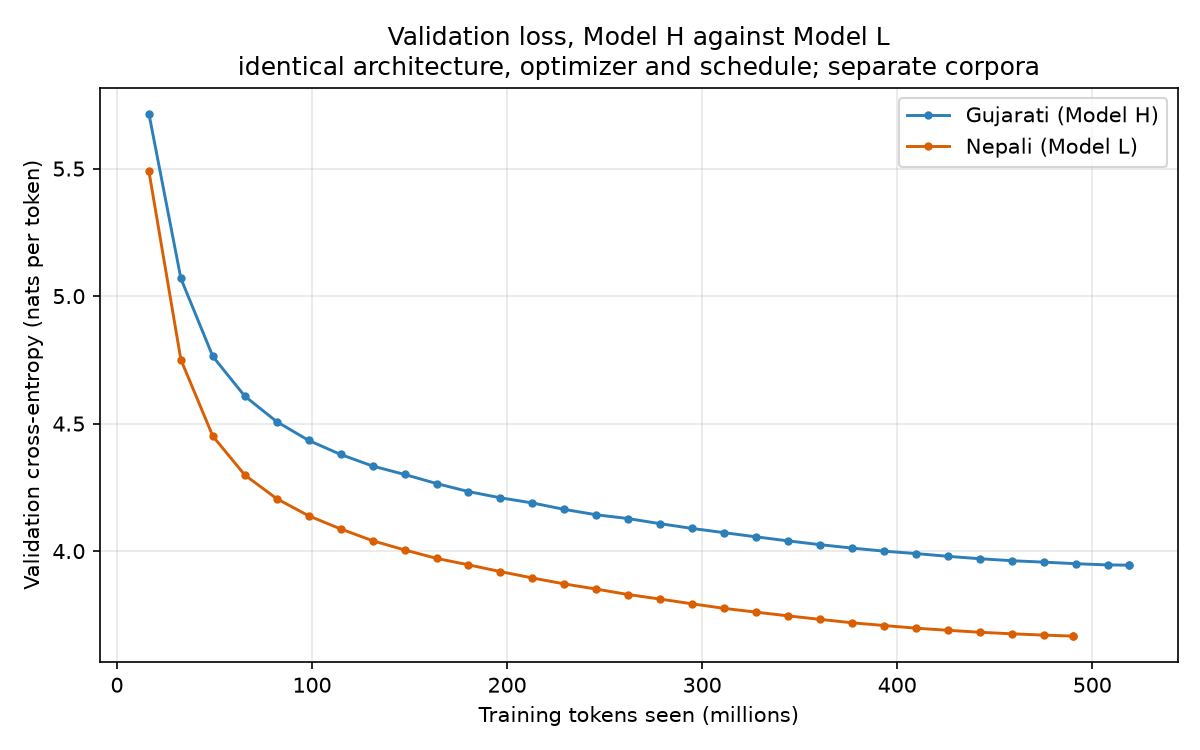
\includegraphics[width=\linewidth]{figures/models/loss_comparison.png}
\caption{Validation loss for both models against tokens seen. Identical architecture, optimizer and schedule; separate corpora. Validation loss tracks training loss throughout, which is the check that zero dropout was the right choice.}
\label{fig:loss}
\end{figure}


\section{Language modelling results}

\begin{table}[H]
\centering
\small
\begin{tabular}{llrr}
\toprule
\textbf{Split} & \textbf{Metric} & \textbf{Gujarati (H)} & \textbf{Nepali (L)} \\
\midrule
Validation & Cross-entropy (nats/token) & 3.9611 & 3.6535 \\
Validation & Perplexity & 52.52 & 38.61 \\
Validation & \textbf{Bits per byte} & \textbf{0.5826} & \textbf{0.4228} \\
Test & Cross-entropy (nats/token) & 3.9439 & 3.6618 \\
Test & Perplexity & 51.62 & 38.93 \\
Test & \textbf{Bits per byte} & \textbf{0.5764} & \textbf{0.4247} \\
Test & Tokens predicted & 28,225,024 & 27,222,016 \\
\bottomrule
\end{tabular}
\caption{Language-modelling metrics on the complete validation and test splits, in float32, over non-overlapping 512-token windows so every token is predicted exactly once.}
\label{tab:lm}
\end{table}



Bits-per-byte is the number to compare. Perplexity is measured per \emph{token},
and the two tokenizers differ: a Nepali token carries about 21\% more characters
than a Gujarati one, so it is the harder prediction. Dividing the same total
likelihood by UTF-8 bytes removes the tokenizer, because bytes are a property of
the text rather than of how it was split.

Model L is ahead on both measures --- test bits-per-byte 0.4247 against
0.5764, 26.3\% lower --- while seeing 5.5\%
\emph{fewer} tokens under an identical recipe. Section~\ref{sec:compare}
explains why.


\section{Generation quality}

\begin{table}[H]
\centering
\small
\begin{tabular}{llrrrrrr}
\toprule
\textbf{Model} & \textbf{Decoding} & \textbf{BLEU-4} & \textbf{chrF++} & \textbf{ROUGE-L} & \textbf{Dist-1} & \textbf{Dist-2} & \textbf{Rep-4} \\
\midrule
Gujarati & greedy & 2.68 & 16.00 & 12.56 & 0.102 & 0.199 & 0.703 \\
Gujarati & temp 0.5 & 3.27 & 19.52 & 14.31 & 0.190 & 0.456 & 0.263 \\
Gujarati & temp 1.0 & 1.78 & 20.13 & 11.66 & 0.428 & 0.856 & 0.003 \\
Gujarati & temp 1.5 & 0.25 & 16.23 & 4.79 & 0.614 & 0.982 & 0.003 \\
Gujarati & \emph{reference} & -- & -- & -- & 0.394 & 0.824 & 0.007 \\
Nepali & greedy & 1.91 & 15.82 & 11.66 & 0.110 & 0.212 & 0.631 \\
Nepali & temp 0.5 & 2.31 & 19.36 & 13.17 & 0.222 & 0.533 & 0.176 \\
Nepali & temp 1.0 & 1.41 & 21.02 & 10.38 & 0.424 & 0.882 & 0.001 \\
Nepali & temp 1.5 & 0.08 & 17.37 & 4.10 & 0.611 & 0.982 & 0.003 \\
Nepali & \emph{reference} & -- & -- & -- & 0.393 & 0.862 & 0.006 \\
\bottomrule
\end{tabular}
\caption{Generation quality on 200 held-out test documents: a 64-token prompt continued for 96 tokens, scored against the true continuation. The held-out reference is scored the same way, so the diversity numbers have a yardstick.}
\label{tab:gen}
\end{table}



\textbf{Which metric is informative.} chrF++ is the useful one here: both
languages mark case and number with suffix chains, so a correct stem with the
wrong ending scores zero on word-level BLEU but keeps most of its character
$n$-grams. BLEU-4 is weak for open-ended continuation --- there is no single
correct next 96 tokens, and exact 4-gram overlap with one reference is close to
accidental --- but its \emph{ranking} across decoding settings is still
meaningful. ROUGE-L sits between them: the longest common subsequence rewards the
right words in the right order without demanding adjacency.

\textbf{What the numbers say.} Greedy decoding collapses into loops, with
repetition-4 at 0.703 (Gujarati) and 0.631 (Nepali) against
about 0.007 for the held-out reference.
Temperature 0.5 is fluent but circles a topic, which is why it scores the best
BLEU-4 and ROUGE-L. Temperature 1.0 reads best and is where chrF++ peaks
(20.13 and 21.02), with diversity almost exactly matching the
reference. Temperature 1.5 breaks down: Distinct-2 reaches 0.982, \emph{above}
the reference, which is the diagnostic that the text has become more varied than
real text.

\textbf{Coherence and language correctness.} Script, morphology, agreement and
punctuation are right far more often than not in both languages. What is missing
is discourse-level consistency: dates, numbers and places are invented, and
consecutive sentences need not be about the same event. That is what a
25M-parameter model trained for one epoch should look like --- local fluency
without long-range factual control.


\subsection{Sample continuation (Gujarati, Model H)}

\textbf{Prompt.} 

\gujaratitext{રોબોટીક સર્જરીમાં દર્દીઓને ઓછો રક્તસ્ત્રાવ, નાના ચીરા અને ઝડપી રિકવરીના લાભો જોવા મળે છે: ડો. અમીષ મહેતા સૌરાષ્ટ્ર અને કચ્છ વિસ્તારમાં કિડની ટ્રાન્સપ્લાન્ટ સહિત કિડની રોગની સંપૂર્ણ સારવાર પૂરી પાડતી ...}





\textbf{Greedy} --- note the loop: 

\gujaratitext{ની જરૂરિયાત ધરાવતા ડો. અમીષ મહેતાએ જણાવ્યું હતું કે, કિડનીની સારવારમાં કિડનીની કામગીરીમાં વધારો થાય છે. કિડનીની કામગીરીમાં વધારો થાય છે. કિડનીની કામગીરીમાં વધારો થાય છે. કિડનીની કામગીરીમાં વધારો થાય છે. કિડનીની કામગીરીમાં વધારો થાય છે. ...}





\textbf{Temperature 1.0:} 

\gujaratitext{માં ૭૨ બેડની , ટિપોરીનની જરૂરિયાત વધુ રખાયેલી ટાંકાઓ, કેટલીક કટ બહેનો તેમજ દર્દીઓ નો સમયસર બને અને દર્દીઓને સમયસર સંકલન અને તેમાં પણ તાત્કાલિક સારવાર મળે એ હેતુથી આવા જટિલ ઓપરેશનનો સાચો ખર્ચ અથવા સર્જરીમાંવાસના સ્થળે જો સાચો અથવા તો કિડની ચોક્કસ નથી તેવું આયોજન કરાયુ છે. વડાપ્રધાન નરેન્દ્રભાઈ ...}




\subsection{Sample continuation (Nepali, Model L)}

\textbf{Prompt.} 

\nepalitext{स्याफ्रुवेसीबाट बिहान साँढे सात बजे निस्कँदा, एकैदिनमा धेरै माथिसम्म नजानु 'हाइ' (लेक) लाग्छ भन्ने लोप्साङ, लामा होटल आइपुग्दा, पानी पर्दैन तपाईहरु माथि जान सक्नुहुन्छ भन्न थालेको थियो। दुई बजे लामा ...}





\textbf{Temperature 1.0:} 

\nepalitext{तल घर तिर लाग्न भनेर घोढिरहेक थियौं। चार्ज गराउन समय निकाले, वन फायल फर्काए। सो क्रममा रैछ म। सबैजना भाग्ने नि कता हो कता ! सेनाले कति जाडोबाट जोगाउनुप}\fallbacktext{¥}\nepalitext{यो, यहाँको शान्त वातावरणले गर्दा हामी सकभर सो बाटोै पारि गाउँ पु}\fallbacktext{¥}\nepalitext{याउँछौं। त्यता तिरबाट बाटोको नजिकै पुग्छौं। बेस्सरी उभिएर हेर्दा मज्जा आउँछ। ...}





More samples, and the same prompts run by hand at three
temperatures, are in \texttt{samples.md} and \texttt{model\_output.md} under
each model's report directory.

\section{Attention analysis}

\begin{table}[H]
\centering
\small
\begin{tabular}{lrr}
\toprule
\textbf{} & \textbf{Gujarati (H)} & \textbf{Nepali (L)} \\
\midrule
Mean normalised entropy & 0.691 & 0.669 \\
Mean attention distance (tokens) & 67.9 & 68.2 \\
Mean previous-token mass & 0.090 & 0.092 \\
Mean start-token (sink) mass & 0.059 & 0.026 \\
Most diffuse layer & L0 (0.918) & L0 (0.946) \\
Most focused layer & L8 (0.471) & L9 (0.459) \\
Longest-range layer & L0 (100.9) & L0 (113.9) \\
\bottomrule
\end{tabular}
\caption{Attention statistics, averaged over 81{,}920 tokens of held-out text. Entropy is normalised by the log of the number of keys visible at that position, so 1.0 means uniform attention at any depth.}
\label{tab:attn}
\end{table}


\begin{figure}[H]
\centering
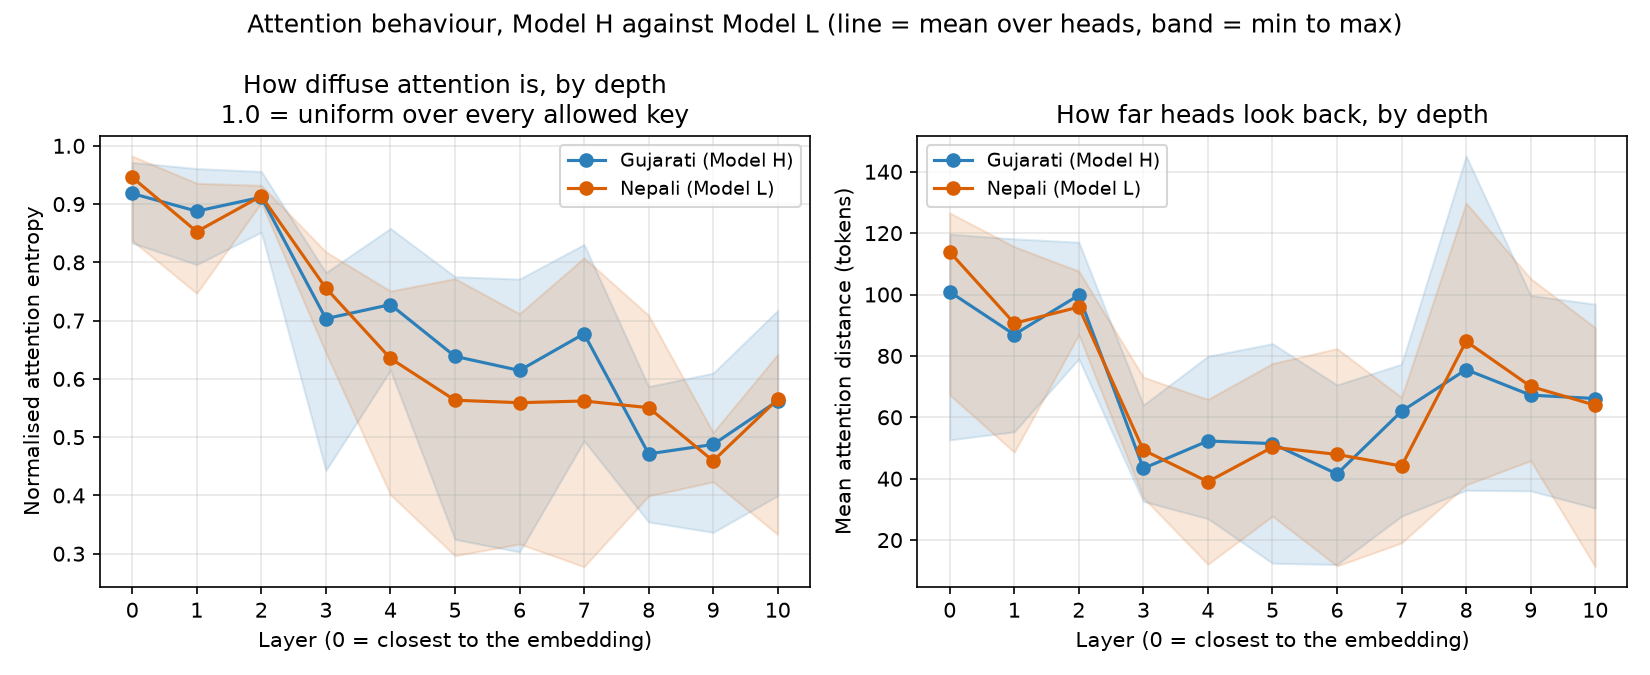
\includegraphics[width=\linewidth]{figures/models/attention_comparison.png}
\caption{Attention behaviour by depth. Line is the mean over heads, band is min to max. Early layers are diffuse and long-range; the middle of the stack is where focused, local heads appear.}
\label{fig:attnprofile}
\end{figure}



Both models arrive at closely matched structure. Layers 0--2 are diffuse and
long-range (normalised entropy 0.85--0.95, mean distance 87--114 tokens): early
attention averages broadly over the prefix rather than selecting from it. Across
layers 3--6 entropy drops to 0.56--0.76 and mean distance to 39--52 tokens, and
individual heads become strongly previous-token --- Gujarati L6H0 puts 58\% of its
mass on exactly $t-1$, Nepali L7H3 puts 58\%. These are the local, positional
heads. Late layers split in two: some stay local (Nepali L10H2 has a mean
distance of 11.3 tokens) while others become long-range and content-driven
(Gujarati L8H1 reaches 145 tokens at low entropy, which is focused attention on
something far back rather than an average).

The clearest difference between the two models is the \emph{attention sink}.
Gujarati parks 5.9\% of its mass on the start token overall and 21\% at layer 8,
with one head at 41.9\%; Nepali parks 2.6\% and never exceeds 10.9\% in any head.
A sink head is one with nothing to contribute at that position, dumping its mass
somewhere harmless. Model H uses that escape route about twice as often, which is
consistent with the more varied corpus it is modelling.


\subsection*{Example sentence --- Gujarati}
\gujaratitext{ગુજરાત સરકારે ૨૦૨૪ના શૈક્ષણિક વર્ષથી રાજ્યની તમામ પ્રાથમિક શાળાઓમાં માતૃભાષામાં શિક્ષણ ફરજિયાત બનાવવાનો નિર્ણય લીધો હતો.}

20 tokens including the leading \texttt{<s>}; the heatmap axes below are indices into this sentence, and the numbered pieces are in \texttt{attention\_examples.md}.


\begin{figure}[H]
\centering
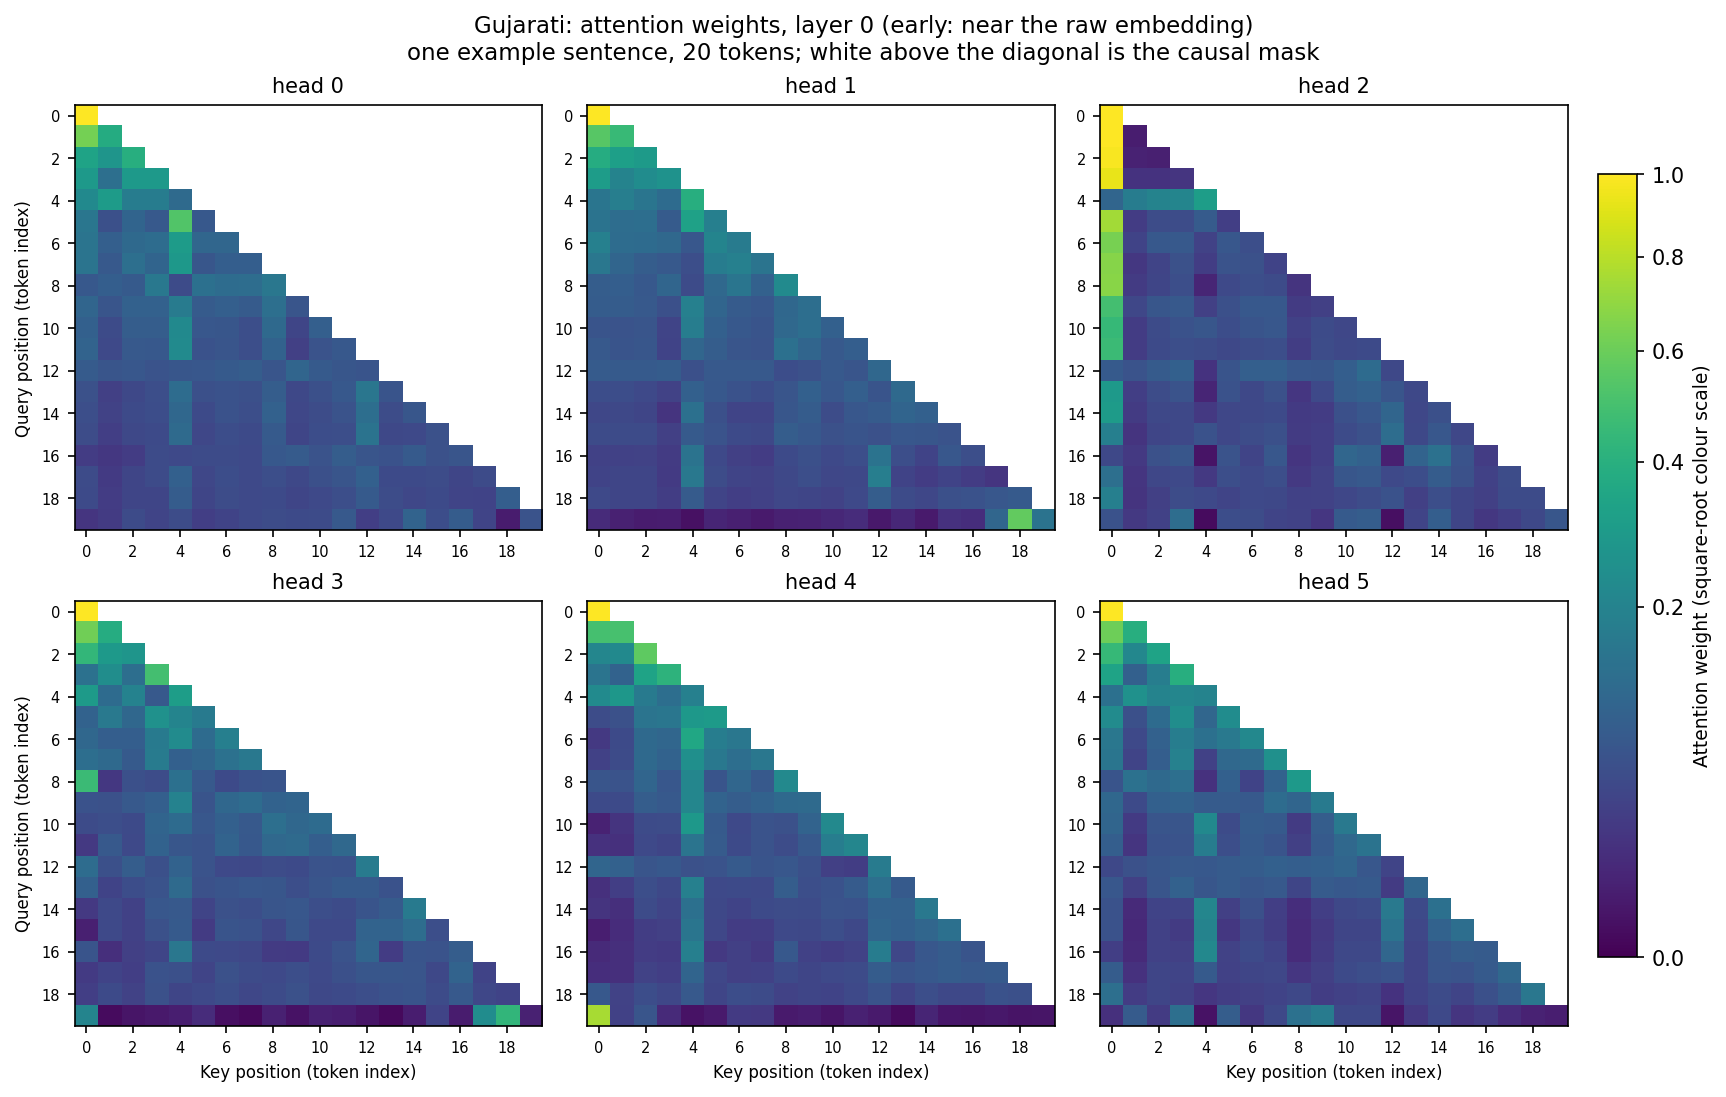
\includegraphics[width=\linewidth]{gujarati/gujarati_16k/figures/attention_example1_layer0.png}
\caption{Gujarati (Model H), \textbf{early layer 0}, all six heads. Axes are token indices; white above the diagonal is the causal mask. The broad triangular wash is the diffuse early-layer behaviour the entropy numbers predict.}
\label{fig:heatgujarati0}
\end{figure}


\begin{figure}[H]
\centering
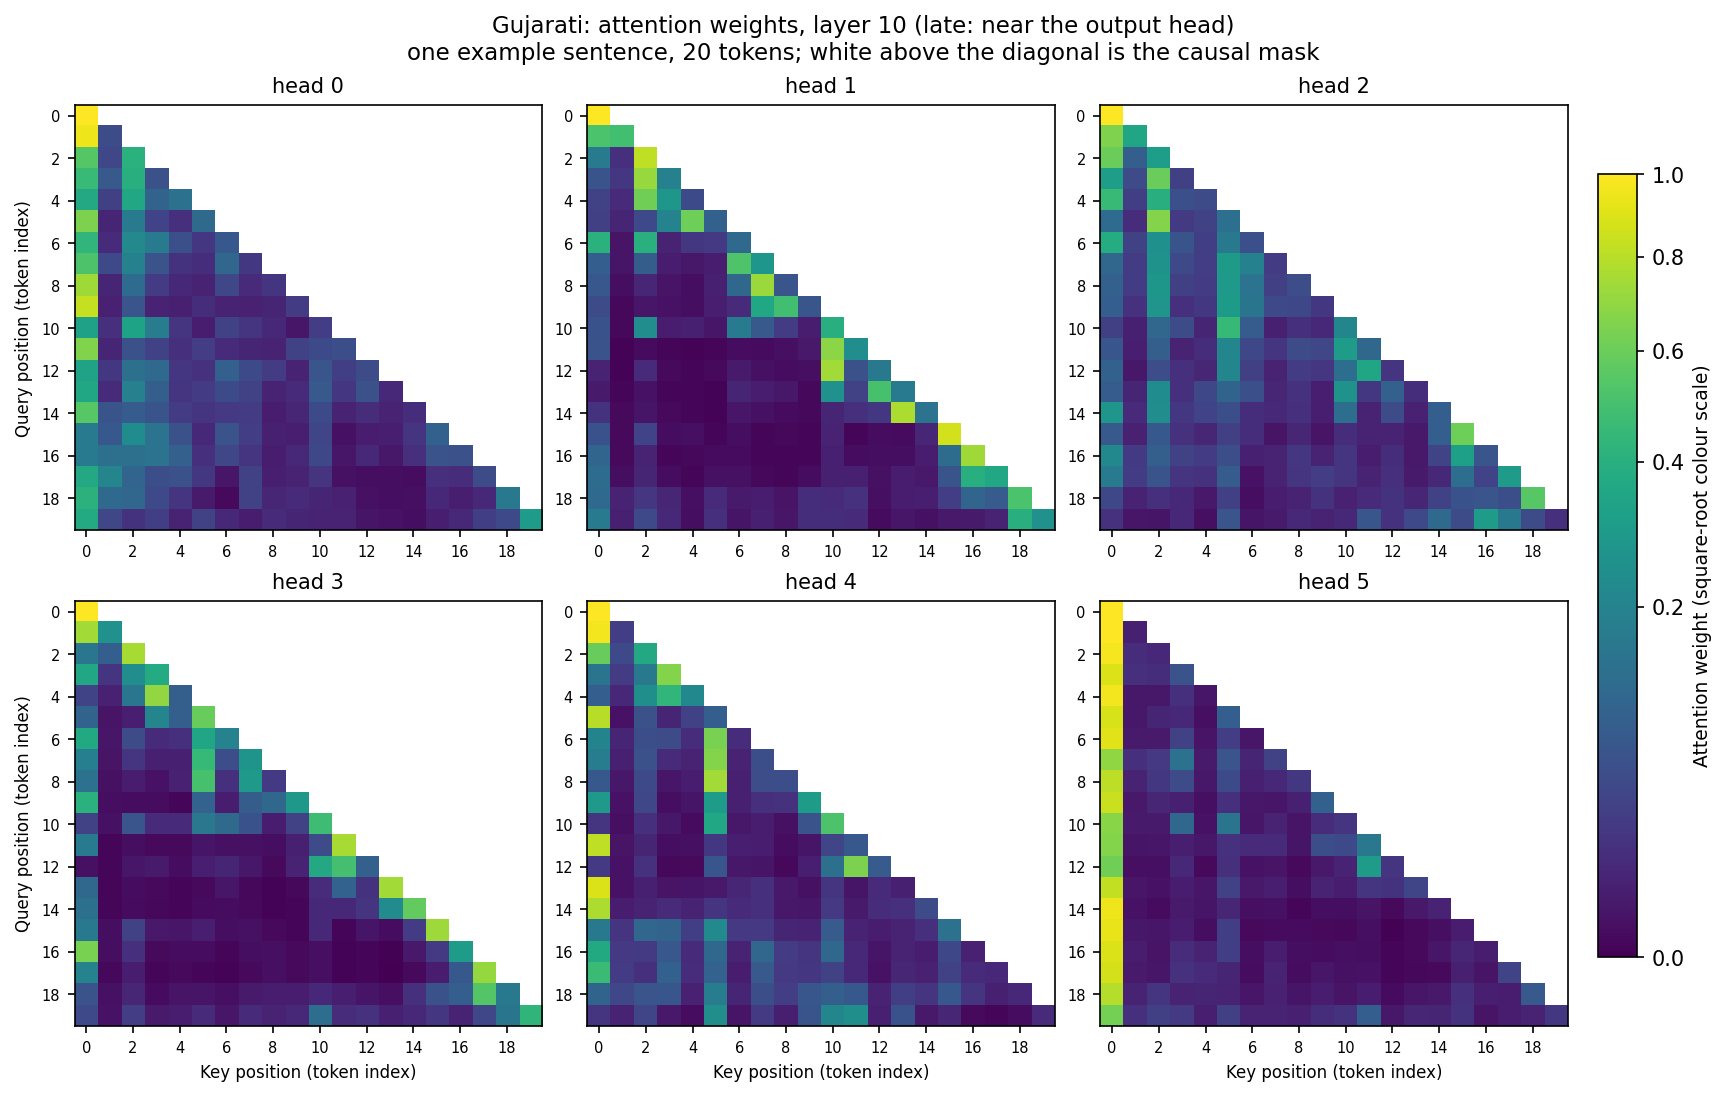
\includegraphics[width=\linewidth]{gujarati/gujarati_16k/figures/attention_example1_layer10.png}
\caption{Gujarati (Model H), \textbf{late layer 10}, all six heads. Narrow near-diagonal bands (local heads) and isolated bright columns far to the left (content-based and sink heads) replace the early wash.}
\label{fig:heatgujaratiL}
\end{figure}


\subsection*{Example sentence --- Nepali}
\nepalitext{नेपाल सरकारले २०८१ सालको बजेटमा शिक्षा र स्वास्थ्य क्षेत्रका लागि छुट्याइएको रकम बढाउने निर्णय गरेको छ।}

18 tokens including the leading \texttt{<s>}; the heatmap axes below are indices into this sentence, and the numbered pieces are in \texttt{attention\_examples.md}.


\begin{figure}[H]
\centering
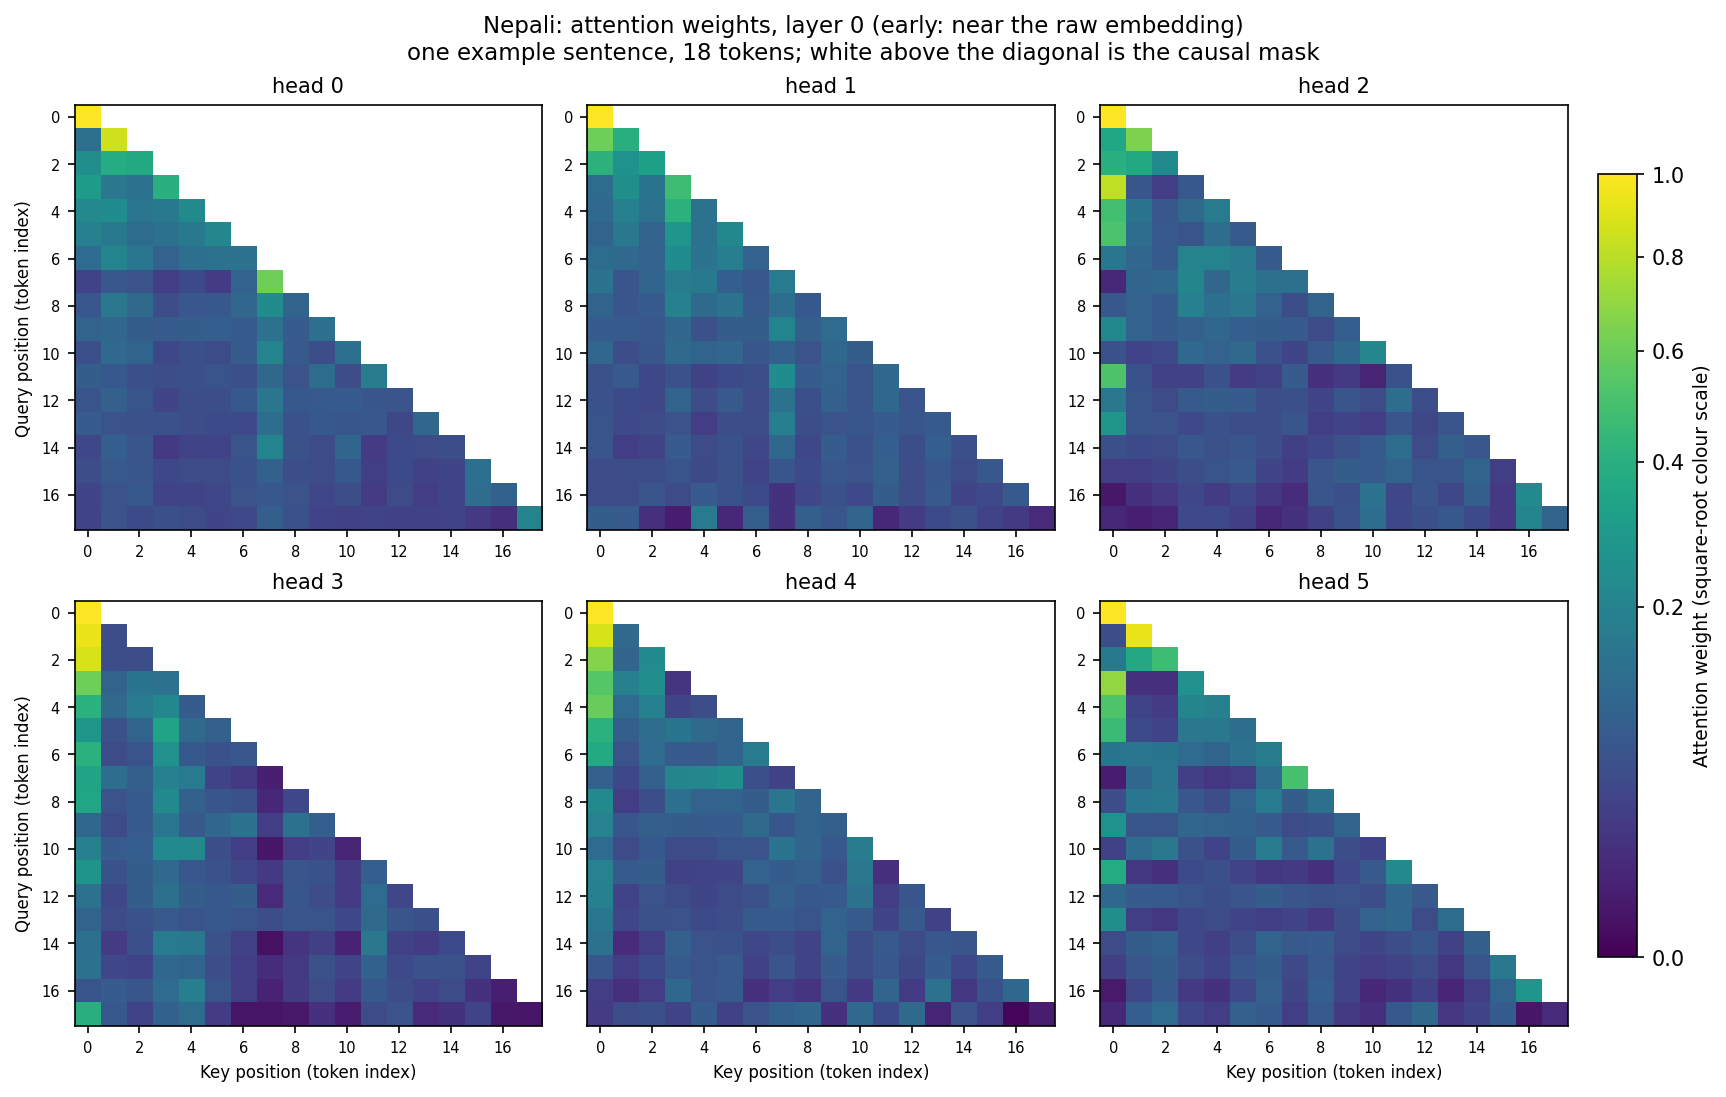
\includegraphics[width=\linewidth]{nepali/nepali_16k/figures/attention_example1_layer0.png}
\caption{Nepali (Model L), \textbf{early layer 0}, all six heads. Axes are token indices; white above the diagonal is the causal mask. The broad triangular wash is the diffuse early-layer behaviour the entropy numbers predict.}
\label{fig:heatnepali0}
\end{figure}


\begin{figure}[H]
\centering
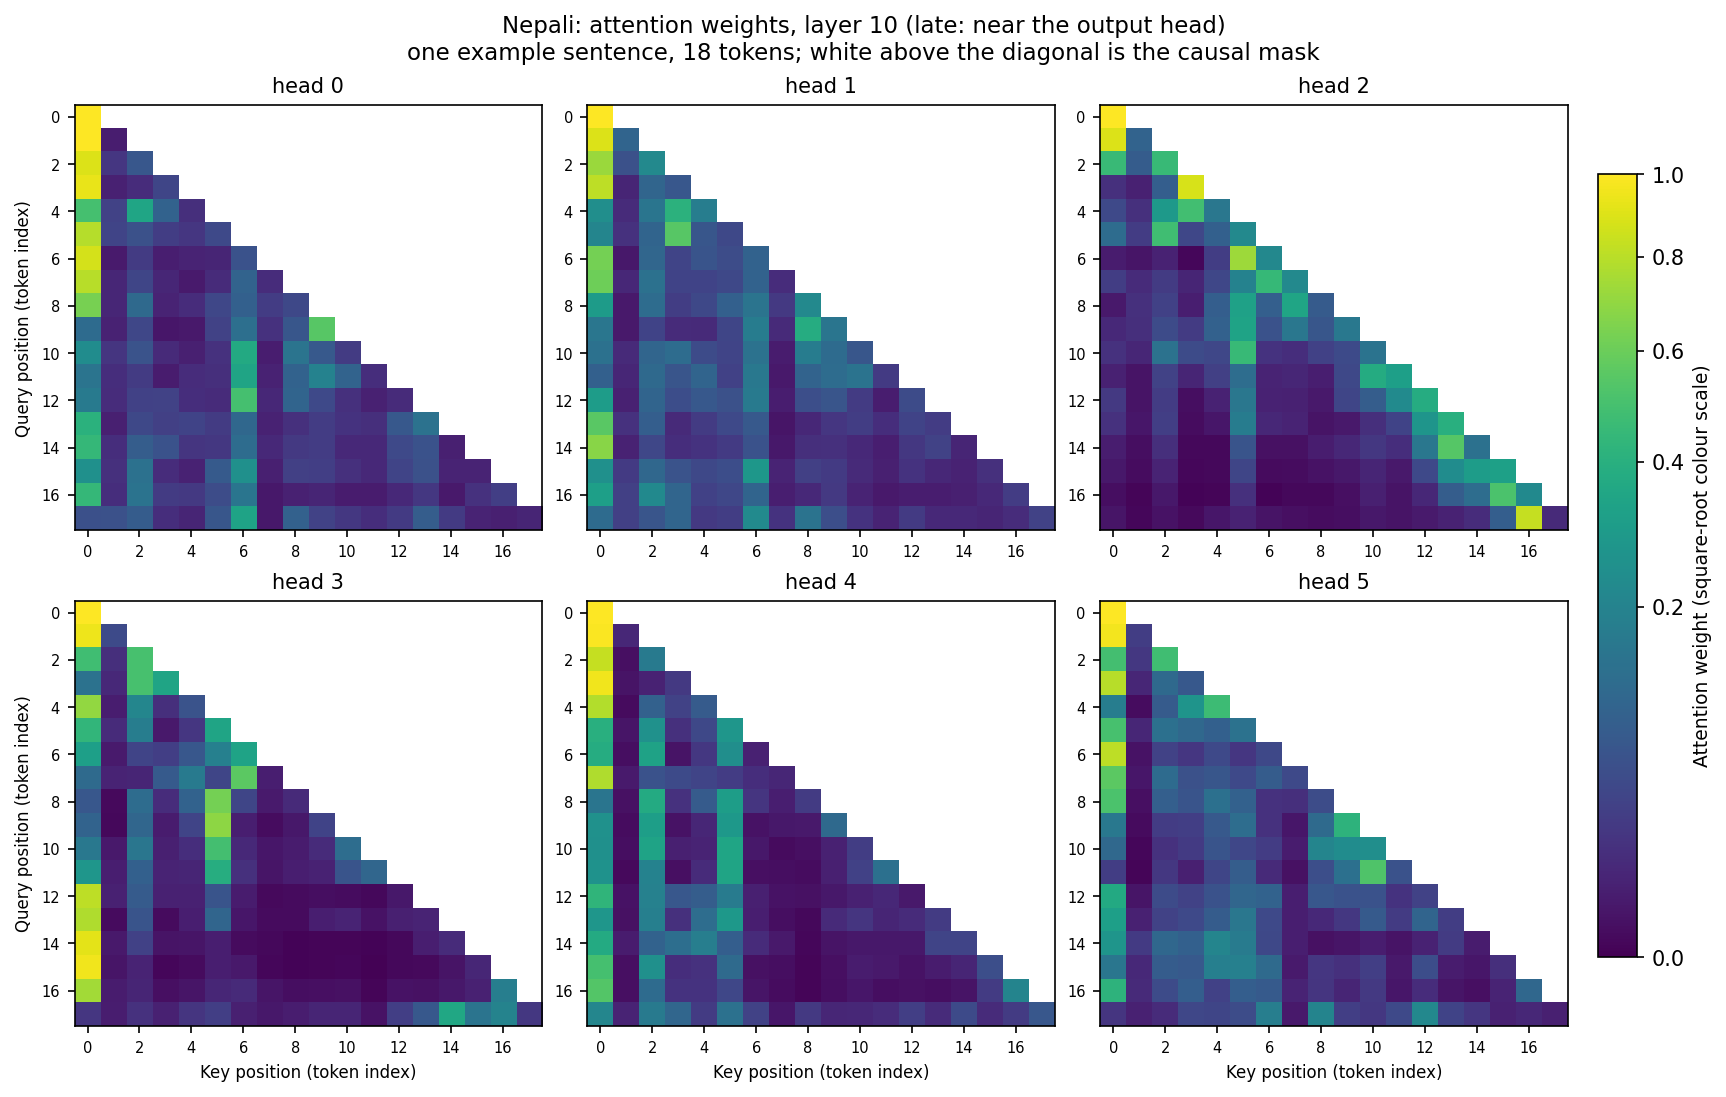
\includegraphics[width=\linewidth]{nepali/nepali_16k/figures/attention_example1_layer10.png}
\caption{Nepali (Model L), \textbf{late layer 10}, all six heads. Narrow near-diagonal bands (local heads) and isolated bright columns far to the left (content-based and sink heads) replace the early wash.}
\label{fig:heatnepaliL}
\end{figure}


\section{Model H against Model L}\label{sec:compare}

\begin{table}[H]
\centering
\small
\begin{tabular}{lrrr}
\toprule
\textbf{} & \textbf{Gujarati (Model H)} & \textbf{Nepali (Model L)} & \textbf{Difference} \\
\midrule
Training tokens & 518,586,368 & 490,274,816 & $-5.5\%$ \\
Manual share of corpus & 31.44\% & 21.58\% & $-9.9$ pts \\
Characters per token & 3.865 & 4.689 & $+21\%$ \\
Fertility (tokens/word) & 1.503 & 1.416 & $-5.8\%$ \\
Sources in the corpus & 1 public + 12 manual & 1 public + 23 manual & -- \\
\bottomrule
\end{tabular}
\caption{The only three things that differ between the two runs: the corpus, its composition, and the tokenizer. Architecture, optimizer, schedule, batch size, epochs and seed are identical. Corpus figures come from Phase 1.}
\label{tab:compare}
\end{table}



The lower-resource model scoring \emph{better} is a statement about the corpora,
not about the two languages or the two networks. Phase 1 measured the difference:
8.7\% of the Gujarati training split is archive.org OCR of books, compressing at
2.77 characters per token against 3.97 for its other manual sources, so Model H
is predicting a more varied and noisier distribution. The Nepali split has no
comparable source and is 78.4\% one homogeneous public corpus, which is easier to
model. Nepali's tokenizer also has better fertility (1.416 tokens per word
against 1.503), so its model spends fewer prediction steps per sentence.

Two effects therefore pull in opposite directions, and both favour Model L: a
more homogeneous corpus and a more efficient tokenizer, against 5.5\% fewer
training tokens. The honest reading is that a single held-out bits-per-byte
cannot separate ``the model learned more'' from ``the held-out text was more
predictable''.


\section{Vocabulary ablation: 16k against 12k}


Phase 1 chose a 16{,}000-piece vocabulary using a rule about parameter budget and
vocabulary coverage, not a measurement of downstream quality. Phase 2 tests that
choice by training the 12{,}000-piece runner-up as well, for both languages, at
the same parameter budget so that vocabulary is the variable and depth absorbs
it.


\begin{table}[H]
\centering
\small
\begin{tabular}{llrrr}
\toprule
\textbf{Model} & \textbf{Metric (test split)} & \textbf{16k} & \textbf{12k} & \textbf{Change} \\
\midrule
Gujarati & Perplexity \emph{(not comparable)} & 51.62 & 44.64 & -13.5\% \\
Gujarati & \textbf{Bits per byte} \emph{(comparable)} & \textbf{0.5764} & \textbf{0.5759} & \textbf{-0.08\%} \\
Gujarati & Wall-clock hours & 4.57 & 5.17 & +13.0\% \\
Nepali & Perplexity \emph{(not comparable)} & 38.93 & 33.47 & -14.0\% \\
Nepali & \textbf{Bits per byte} \emph{(comparable)} & \textbf{0.4247} & \textbf{0.4236} & \textbf{-0.26\%} \\
Nepali & Wall-clock hours & 4.51 & 4.91 & +8.9\% \\
\bottomrule
\end{tabular}
\caption{Vocabulary ablation at a matched parameter budget: the smaller embedding frees 1.54M parameters, which buys a twelfth Transformer block (25{,}860{,}864 against 25{,}625{,}856, within 0.92\%). Perplexity appears to improve by 13--14\%, but that is the vocabulary changing, not the model.}
\label{tab:ablation}
\end{table}


\begin{figure}[H]
\centering
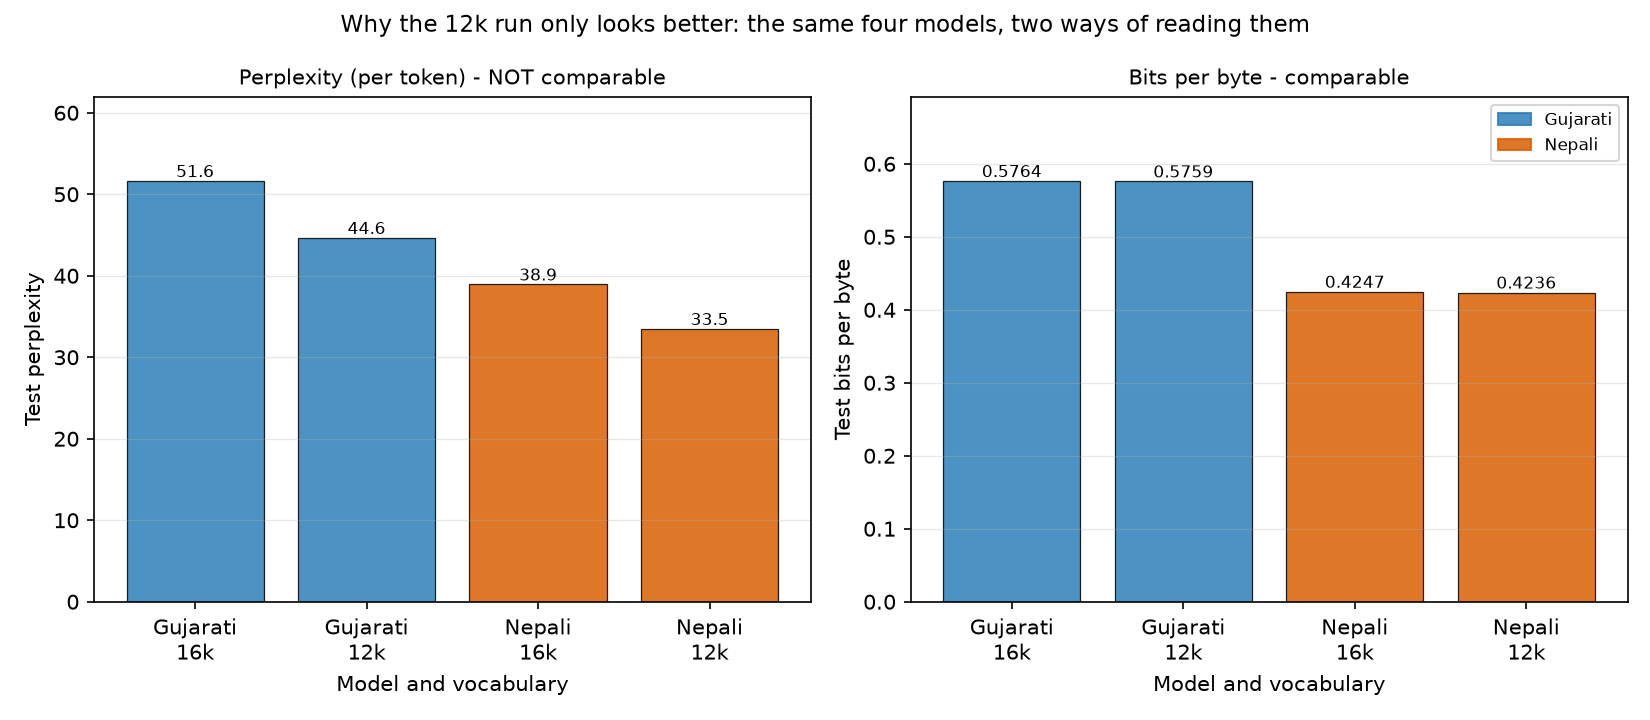
\includegraphics[width=\linewidth]{figures/vocab_ablation/perplexity_vs_bpb.png}
\caption{The same four models read two ways. Perplexity (left) says the 12k runs are much better; bits-per-byte (right) says the two vocabularies are within a fraction of a percent. Only the right panel is a claim about the model.}
\label{fig:trap}
\end{figure}



\textbf{Conclusion.} The Phase 1 choice stands. A 12{,}000-piece vocabulary buys
0.08--0.26\% of bits-per-byte and costs 8.9--13.0\% more wall-clock time per
epoch, for two compounding reasons: the same corpus becomes 3.7--4.0\% more
tokens to read, and every one of those tokens passes through 12 blocks instead of
11. Generation quality does not move in its favour either (chrF++ at the best
decoding setting is flat to slightly worse). The 16k run therefore remains the
reported Phase 2 model and the checkpoint Phase 3 finetunes from.

The result worth keeping is methodological. A 13--14\% perplexity drop that
survives no correction for tokenization is easy to claim and easy to believe.
Bits-per-byte is what separates it from a real improvement, which is why the
brief asks for it.


\section{Reproducing}


\begin{verbatim}
cd gujarati                              # or nepali
python3 model/transformer.py --self-test # RoPE, attention, masking, init
python3 model/param_budget.py            # parameter count, formula vs model
python3 eval/text_metrics.py --self-test # BLEU / chrF vs sacrebleu
python3 train/prepare_data.py            # splits -> uint16 token streams
python3 train/pretrain.py                # pretrain (resumable; --max-hours)
python3 eval/run_eval.py                 # the whole evaluation suite
python3 report/phase2/make_report_assets.py
\end{verbatim}

Checkpoints (${\sim}295$ MB per run) are published at
\url{https://huggingface.co/hardik300/LMA\_mini\_project}, one folder per run,
with the link also in the top-level \texttt{README}; training logs, loss curves,
evaluation JSON, generated samples and attention figures are committed under
\texttt{<language>/logs/pretrain/} and \texttt{report/phase2/}. Full tables are in
\texttt{report/phase2/results.md} and \texttt{report/phase2/vocab\_comparison.md};
this report is generated from the same JSON by
\texttt{report/phase2/make\_report\_pdf.py}.


\end{document}